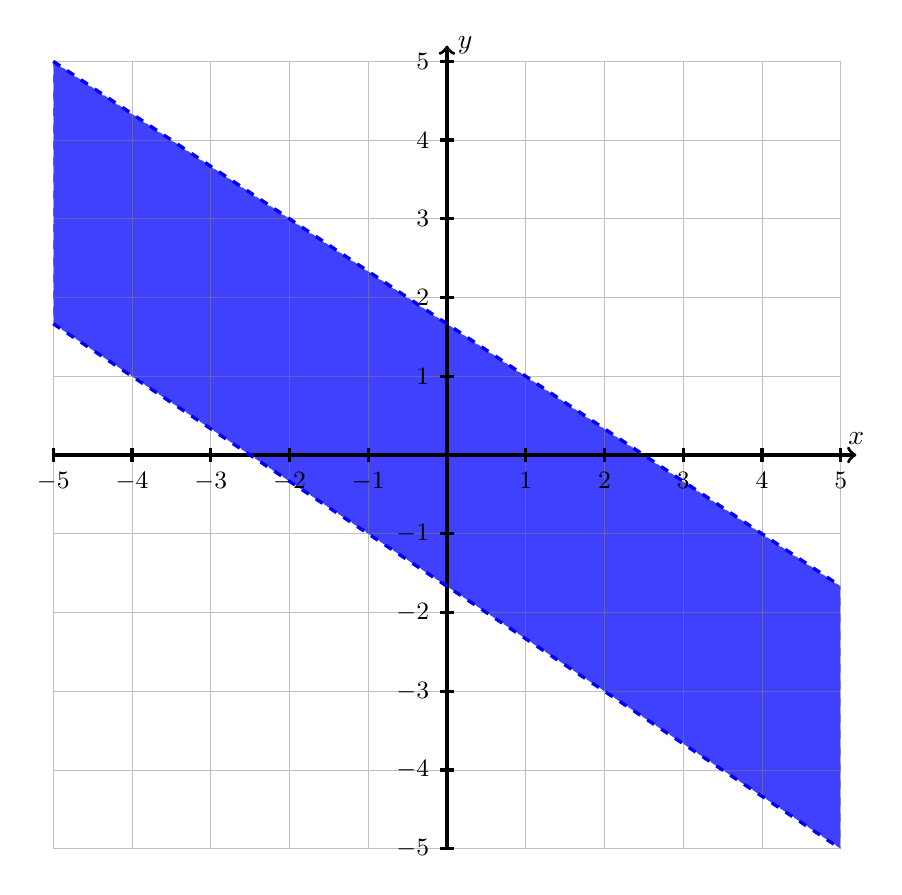
\begin{tikzpicture}
  \def\size{5}

  \draw [color=white, fill=blue,dashed,opacity=.75] (-5,5/3) -- (-5,5) -- (5,-5/3) -- (5,-5) -- (-5,5/3);
  
  \path [draw, help lines, opacity=.5]  (-\size,-\size) grid (\size,\size);
  \foreach \i in {1,...,\size} 
  \draw [very thick] (\i,2.5pt) -- +(0,-5pt) node [anchor=north, font=\small] {$\i$}
  (-\i,2.5pt) -- +(0,-5pt) node [anchor=north, font=\small] {$-\i$} 
  (2.5pt,\i) -- +(-5pt,0) node [anchor=east, font=\small] {$\i$}
  (2.5pt,-\i) -- +(-5pt,0) node [anchor=east, font=\small] {$-\i$};
  \draw [very thick,->] (-\size,0) -- (\size+.2,0) node [anchor=south] {$x$};
  \draw [very thick,->] (0,-\size) -- (0,\size+.2) node [anchor=west] {$y$};

  %% 2x + 3y = -5
  \draw[very thick,blue,dashed] (-5,5/3) -- (5,-5);
  %% 2x + 3y = 5
  \draw[very thick,blue,dashed] (-5,5) -- (5,-5/3);
  
\end{tikzpicture}
